\NTXDivider{Education is Changing}

\begin{frame}{Neuromatch: changing who can learn the methods}
  \begin{columns}[c,onlytextwidth]
    \column{.46\textwidth}
      \small
      \NTXPoint{An open curriculum}{Computational neuroscience, deep learning, and NeuroAI beyond a single university.}
      \NTXPoint{Learning with other people}{Coding, teaching-assistant support, and shared projects.}
      \NTXPoint{An opportunity for our chapters}{Study groups that carry shared learning into local projects.}
    \column{.50\textwidth}
      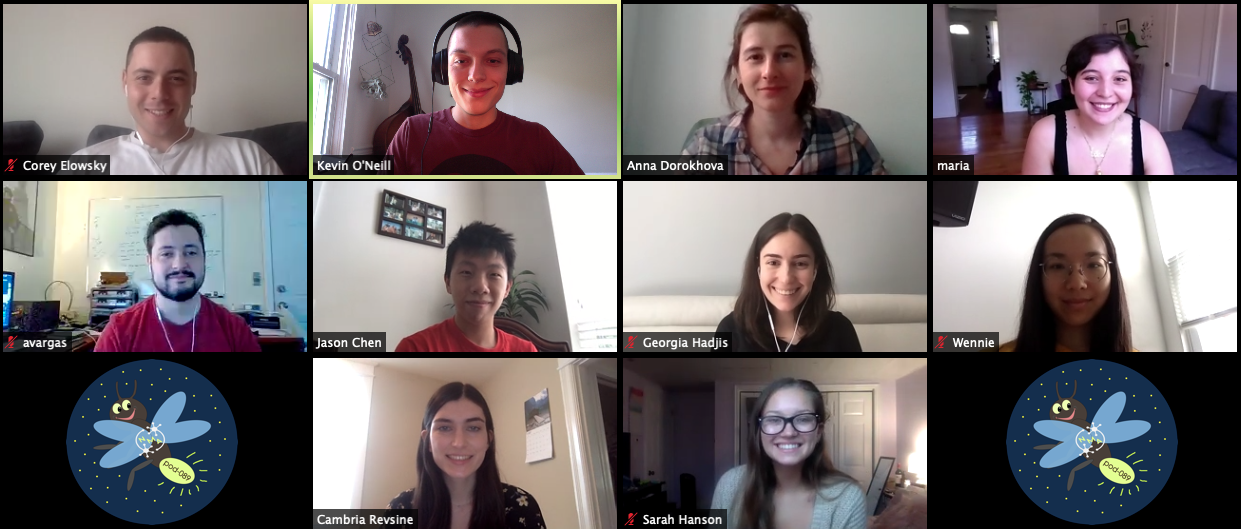
\includegraphics[width=\linewidth,height=44mm,keepaspectratio]{assets/history/neuromatch-pod-2020.png}
      \par\smallskip{\scriptsize Neuromatch Academy, 2020\newline Pod 089 --- photo: \href{https://kevingoneill.github.io/teaching/2020-07-NMA}{Kevin O'Neill}\par}
  \end{columns}
  {\tiny\color{NTXMuted}Sources: \href{https://neuromatch.io/courses/}{Neuromatch courses}; \href{https://neuromatch.io/open-education-resources/}{open educational resources}\par}
  \note{[83:15--85:15] Neuromatch illustrates how a community can make advanced computational education accessible beyond a local department. Distinguish freely available course materials from admission to supported live courses. Its resources are shared for reuse with attribution; external study groups are not automatically Neuromatch-endorsed. The chapter study-group idea is our proposed use, not a new partnership. Connect this to Queen's: complementary routes through structured credentials, open curricula, and peer learning.}
\end{frame}

\begin{frame}{The BCI Guys: another way into neurotechnology}
  \begin{columns}[c,onlytextwidth]
    \column{.52\textwidth}
      \small
      \NTXPoint{Learning through media}{Videos, conversations, and hands-on demonstrations make neurotechnology approachable.}
      \NTXPoint{Foundations of Neurotechnology}{A course developed with NeuroTechX, connecting video learning with NeuroTechEDU materials.}
      \NTXPoint{Why science storytelling matters to me}{I sponsor PBS Space Time and am a major fan of Journey to the Microcosmos.}
    \column{.44\textwidth}
      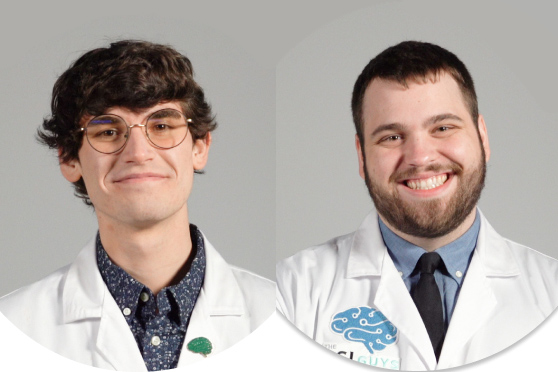
\includegraphics[width=\linewidth,height=39mm,keepaspectratio]{assets/history/bci-guys-rit.jpg}
      \par\smallskip{\scriptsize Harrison Canning and Colin Fausnaught\newline Photo: RIT, 2021\par}
  \end{columns}
  {\tiny\color{NTXMuted}Sources: \href{https://www.bciguys.com/course}{The BCI Guys: course}; \href{https://www.rit.edu/news/rit-student-and-alumnus-follow-passion-neurotechnology}{RIT profile / photograph}\par}
  \note{[85:15--86:45] The BCI Guys offer another entry point: approachable science communication and demonstrations alongside a structured introductory course. Their own 2023 post credits The BCI Guys and NeuroTechX with creating Foundations of Neurotechnology. The course page also describes NeuroTechEDU materials; do not promise that every historical platform remains available. Harrison is pictured left and Colin right. These formats complement formal education and research training. My sponsorship of PBS Space Time and enthusiasm for Journey to the Microcosmos are personal statements, not NeuroTechX sponsorships or partnerships. The lesson is that people can discover the field through compelling content, then find peers and projects through the community.}
\end{frame}

\begin{frame}{MedARC and Sophont: open collaboration in deep learning}
  \begin{columns}[c,onlytextwidth]
    \column{.51\textwidth}
      \small
      \NTXPoint{Research beyond a single lab}{Open medical AI projects, journal clubs, and shared resources.}
      \NTXPoint{A concrete neurotech example}{MindEye and MindEye2: collaborative fMRI-to-image research with public code.}
      \NTXPoint{Community alongside a company}{Sophont connects researchers with MedARC's community and research resources.}
    \column{.44\textwidth}
      \centering
      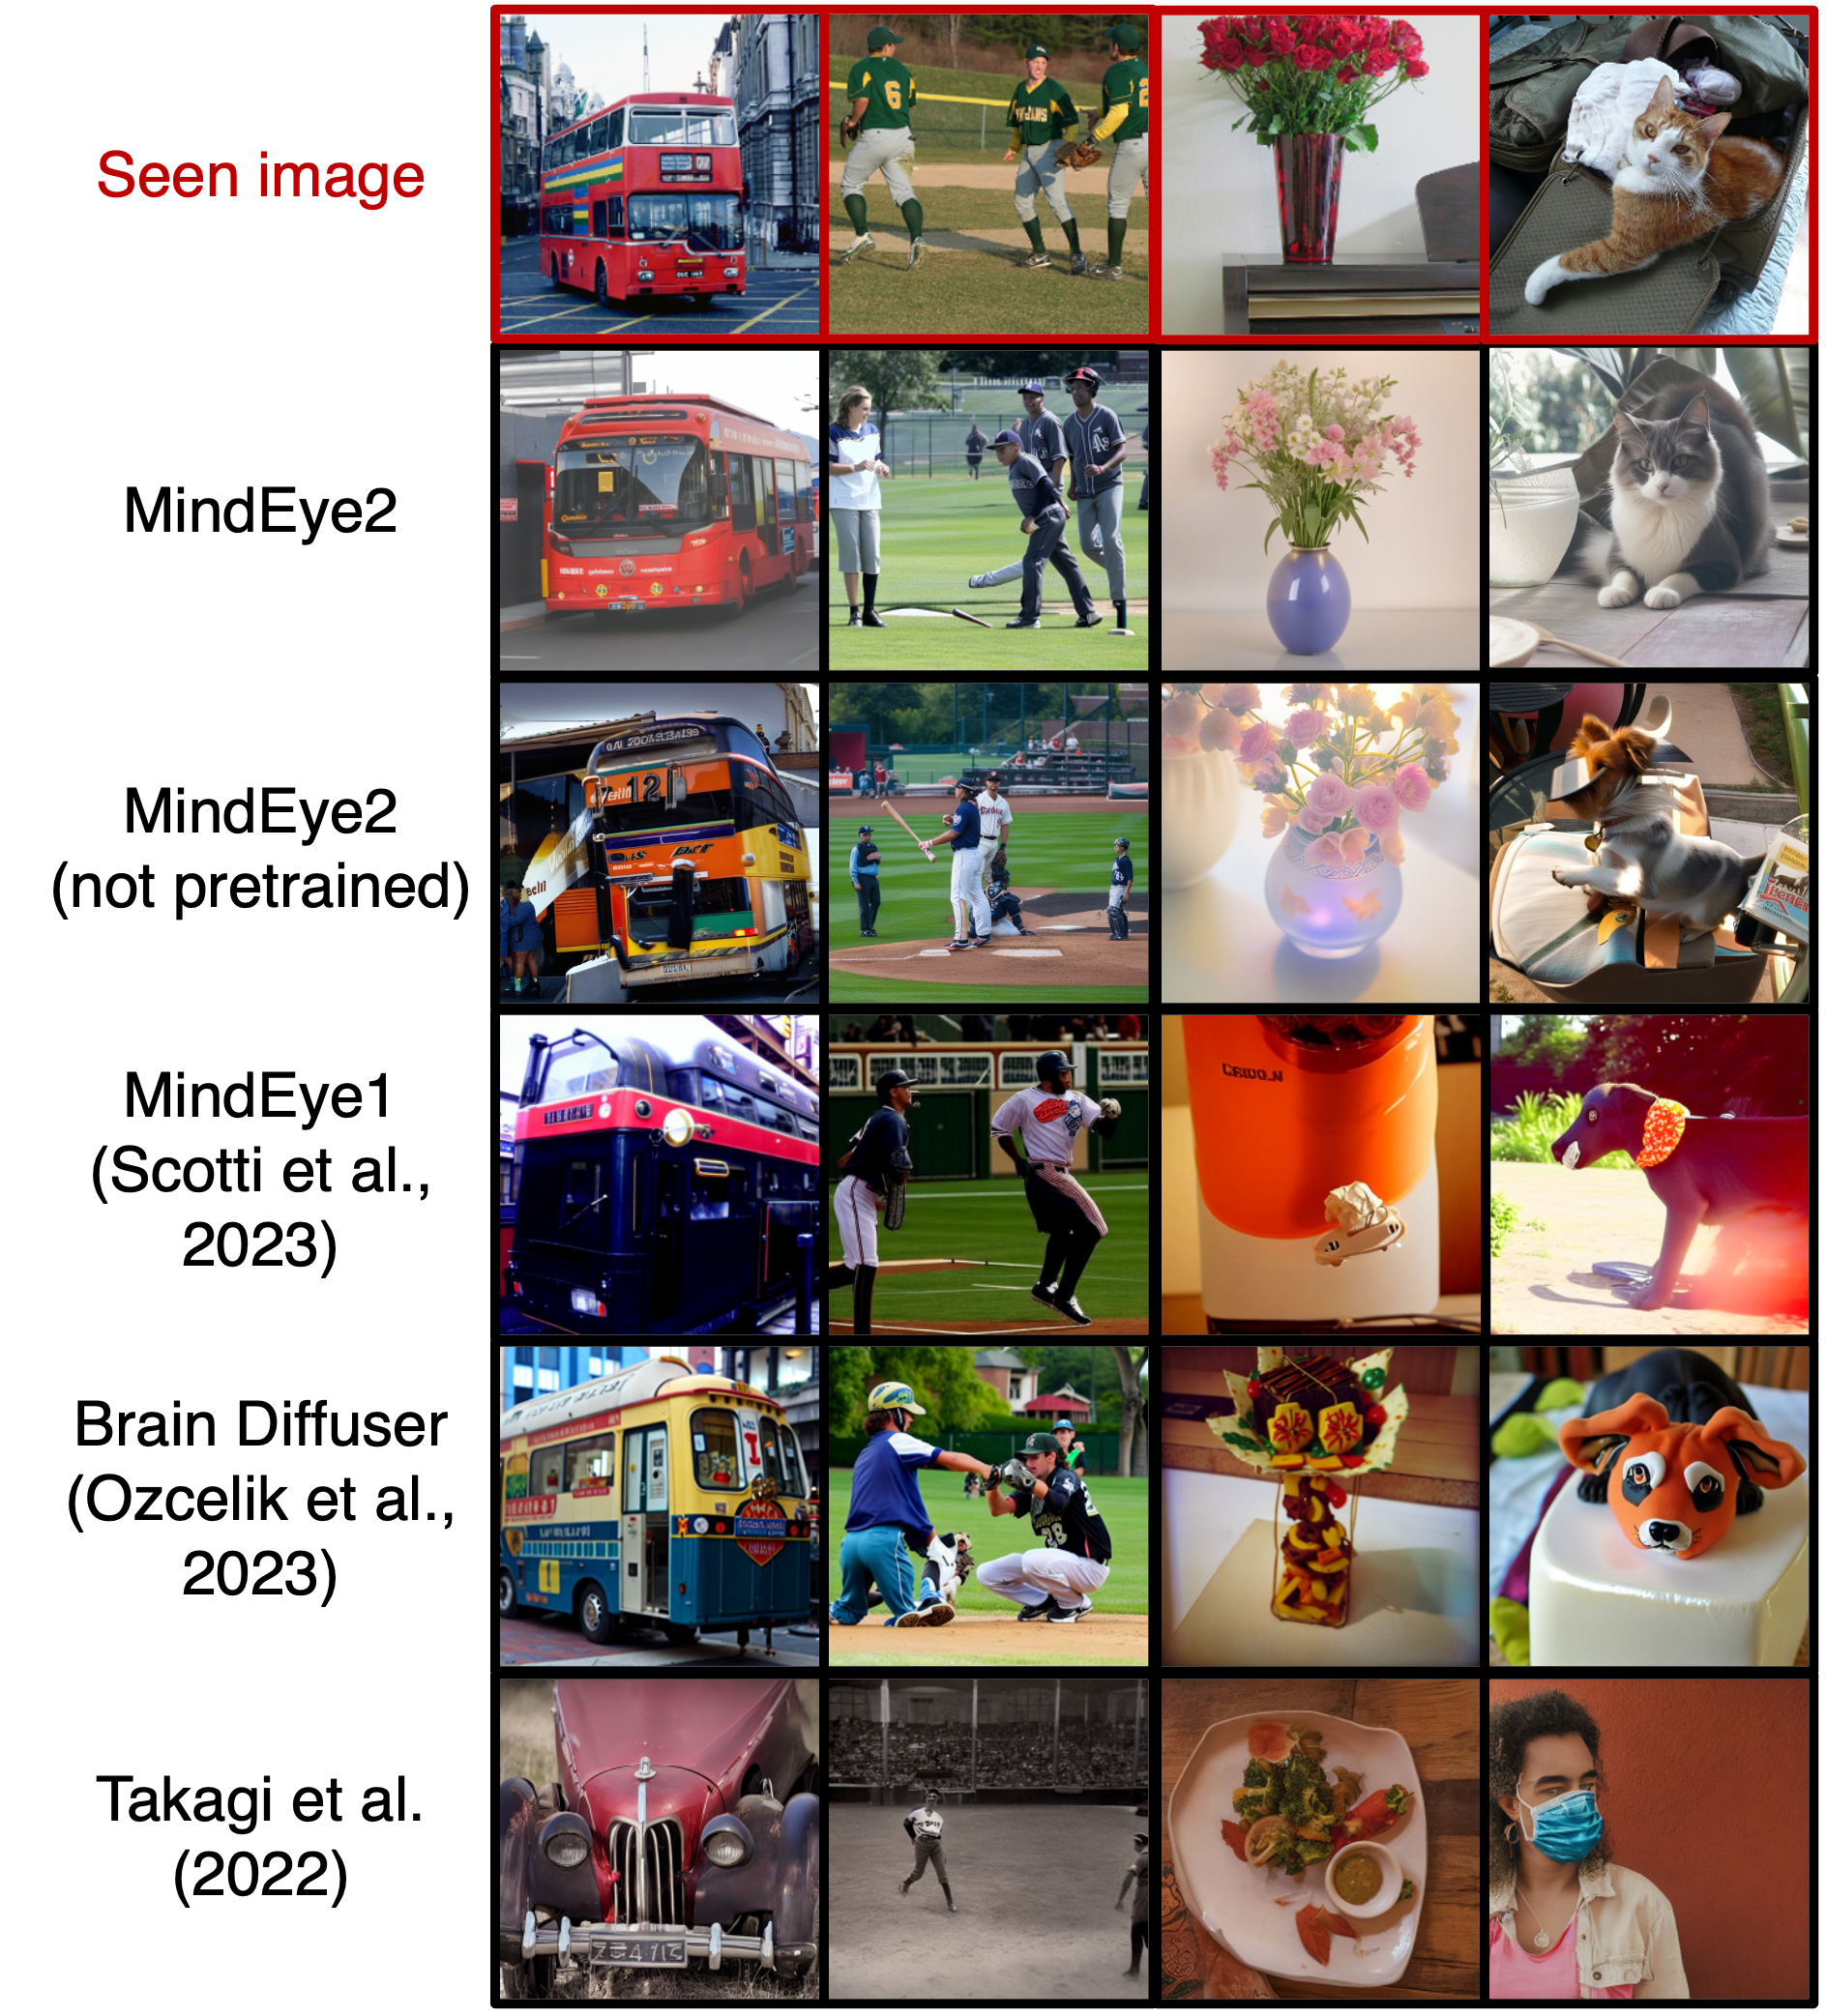
\includegraphics[width=\linewidth,height=46mm,keepaspectratio]{assets/history/medarc-mindeye2-results.png}
      \par\smallskip{\scriptsize MindEye2 --- published reconstruction examples\par}
  \end{columns}
  {\tiny\color{NTXMuted}Sources: \href{https://www.medarc.ai/}{MedARC}; \href{https://sophont.med/}{Sophont}; \href{https://medarc-ai.github.io/mindeye2/}{MindEye2}\par}
  \note{[86:45--88:45] The lesson is an organizational model for participating in deep-learning research: shared projects, expertise, resources, and public research artifacts. Sophont describes these community activities on its own site; access is not a guaranteed entitlement for every volunteer. MindEye2 concerns fMRI-to-image research under a particular experimental setup, not unrestricted mind reading or a consumer device. Do not imply all company assets or datasets are unrestricted. These are external examples, not NTX programs. Ask what our chapters can learn from this way of organizing research.}
\end{frame}

\begin{frame}{Agentic coding: Better Code, Better Science}
  \begin{columns}[c,onlytextwidth]
    \column{.46\textwidth}
      \NTXPoint{Russell A. Poldrack}{An open textbook on reproducible scientific software in the age of AI.}
      \NTXPoint{Beyond generating code}{Testing, workflows, and scientific validation.}
      \NTXPoint{For our community}{Shared reading and code review alongside hands-on projects.}
    \column{.49\textwidth}
      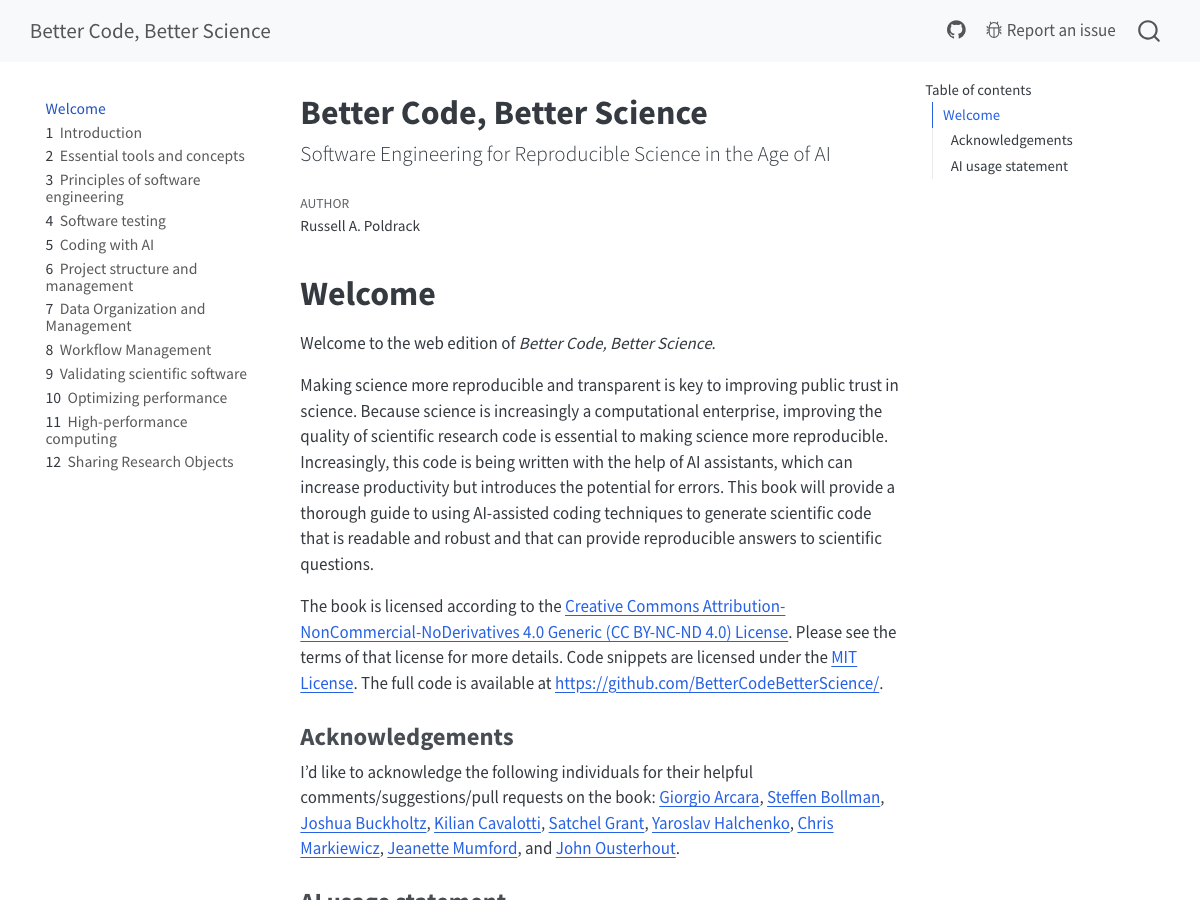
\includegraphics[width=\linewidth,height=48mm,keepaspectratio]{assets/history/better-code-better-science.png}
      \par\smallskip{\scriptsize Official web edition --- title-page screenshot\par}
  \end{columns}
  \NTXSource{https://bettercode-book.org/}{Russell A. Poldrack: Better Code, Better Science; text CC BY-NC-ND 4.0}
  \note{[88:45--89:45] Poldrack introduced this living textbook in May 2025. Its current web edition explicitly addresses readable, robust, reproducible scientific code in the age of AI. Chapters cover software engineering, testing, AI-assisted coding, workflows, and scientific validation. The image is a genuine screenshot of the official web title page, not a fabricated printed-book cover; no official cover was found in the current repository assets. Narrative text is licensed CC BY-NC-ND 4.0 and code snippets MIT. The proposal for NTX reading groups and code review is our suggested use, not a partnership or a course already launched.}
\end{frame}

\begin{frame}{Agentic research: learning the whole workflow}
  \begin{columns}[c,onlytextwidth]
    \column{.52\textwidth}
      \NTXPoint{Seyed Yahya Shirazi, Ph.D.}{Swartz Center for Computational Neuroscience, UC San Diego.}
      \NTXPoint{Agentic Research Course}{A ten-week course hosted by the Open Science Collective; open materials, CC BY 4.0.}
      \NTXPoint{From Git to research practice}{Coding agents, code quality, literature, manuscripts, figures, and neuroinformatics.}
    \column{.43\textwidth}
      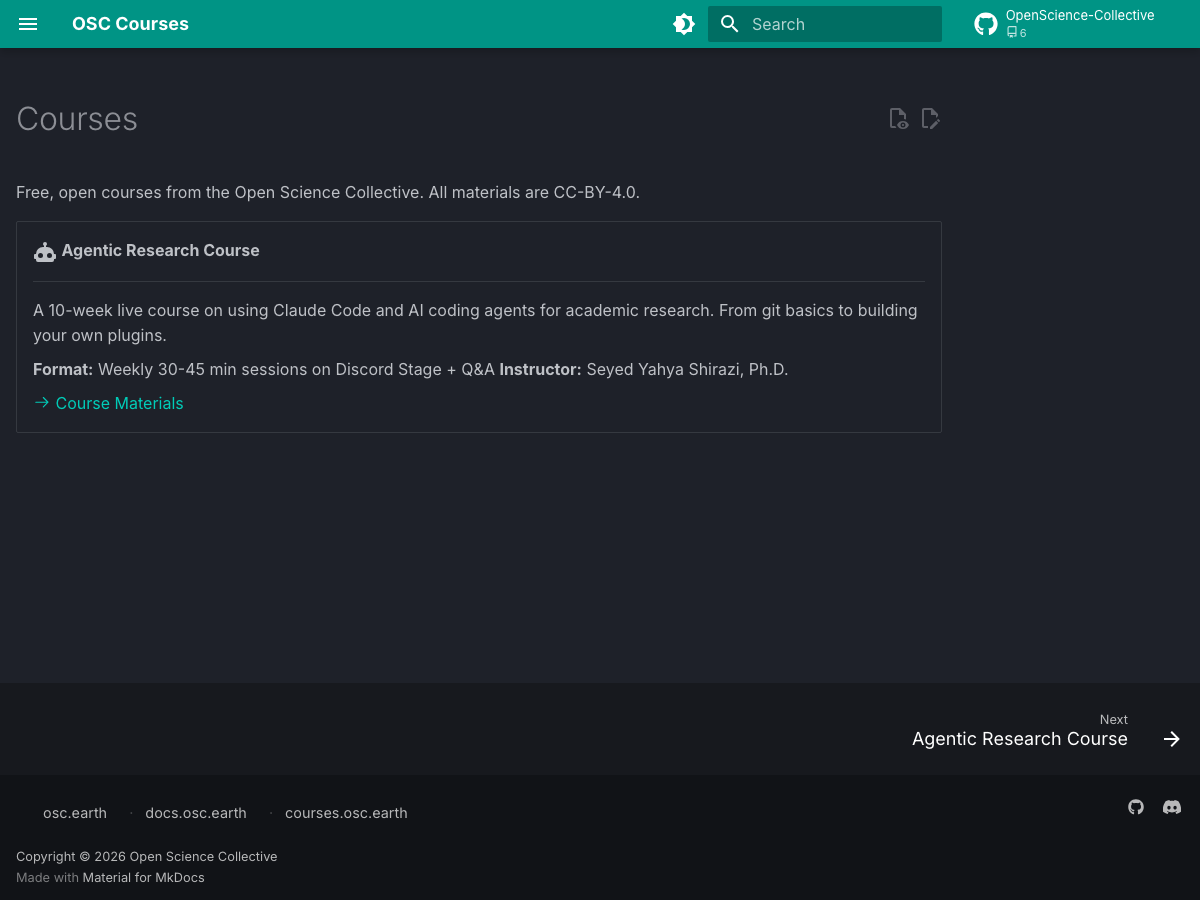
\includegraphics[width=\linewidth,height=44mm,keepaspectratio]{assets/history/agentic-research-course.png}
      \par\smallskip{\scriptsize Official Open Science Collective course page\par}
  \end{columns}
  {\tiny\color{NTXMuted}Sources: \href{https://courses.osc.earth/}{course site / screenshot}; \href{https://github.com/OpenScience-Collective/agentic-research-course}{syllabus, April--June 2026}; \href{https://neuromechanist.github.io/}{instructor}\par}
  \note{[89:45--90:45] This is the course Morgan referred to: Agentic Research Course, taught by Seyed Yahya Shirazi, a researcher at UCSD's Swartz Center for Computational Neuroscience. It is hosted by the Open Science Collective, not presented as a UCSD degree-credit offering. The repository schedules ten sessions from April 8 through June 9, 2026, covering Git, Claude Code, project management, CI/CD, literature search, grants, manuscripts, figures, neuroinformatics, and plugins. The syllabus lists BIDS, PsychoPy, and LSL in its neuroinformatics session. Course materials are free and CC BY 4.0; this does not mean commercial model usage is free. The repository limits its no-prior-coding prerequisite statement to weeks one and two. Do not promise recordings for every session or describe the spring schedule as upcoming. The link is a resource chapters could learn from, not a formal NTX partnership.}
\end{frame}

\NTXDivider{Take Away}
